%\chapter{3HDM}
%\label{ch:3HDM}

\newpage 


\chapter{3HDM}

\section{ The parameter }

something 

\section{Pre-3HDM}

The properties of the new resonance observed at the LHC in 2012 \cite{Aad_2012,chatrchyan2012observation} seem tantalizingly close to those of the Higgs boson predicted by the Standard Model (SM) (for instance, see \cite{collaborations2015combined,collaborations2016measurements} ) 

  
Typical BSM scenarios that aim to fix one or more such shortcomings of the SM often end up extending the scalar
sector of the SM. In these extensions, the 125 GeV scalar observed at the LHC is not the only scalar in the spectrum but the first one in a series of others to follow.

This is an intriguing possibility which motivates us
for a closer inspection of the properties of the observed scalar and inspires us to carry on our efforts to look for
new resonances at the collider experiments.

This is often done by adding to the SM simple replicas of the SM doublet, without altering the EW VEV. The first, and unsurprisingly simplest, of these kinds of models was presented in 1973 in \cite{lee1973theory}, as a means to obtain a spontaneous breaking of the CP symmetry, and boast a rich phenomenology. Along with richer phenomenology the existence of a charged Higgs Boson allows for other phenomena to occur. {\color{red} Explain} 

\section{BGL? Should I meantion it}

The BGL model was a version of one of these 2HDM models where the scalar interactions with fermions explicitly violate flavour families. This akin to what the W boson does on the SM. This is usually avoided trough the creation of a additional $\mathrm{Z}_2$  or a $\mathrm{U}_1$ symmetry [
% S. L. Glashow and S. Weinberg, Natural Conservation Laws for Neutral Currents, Phys. Rev. D15 (1977) 1958.
% E. A. Paschos, Diagonal Neutral Currents, Phys. Rev. D15 (1977) 1966.
% R. D. Peccei and H. R. Quinn, CP Conservation in the Presence of Instantons, Phys. Rev. Lett. 38 (1977) 1440–1443
]. This forces each fermion of the same charge to couple to a single doublet, thereby preventing FCNC.

We already discussed some of the reasons why these symmetries are imposed. These tree-level mediated FCNCs would make significant contributions to the flavour sector observables, such as meson masses or the flavour decays and ratios. This would destroy the agreement with experimental observations. 

Unless the masses of the new scalars are all of order TeV, or the FCNC Yukawas couplings are fine-tuned to be very small. 

These models are meantioned here for the simple fact they propose the reason why the flavour observables are suppresed is through a aditional impossed symmetry. Thus providing a natural explination to why NP contributions to the flavour observables are to be in agreement with the SM. 

\subsection{Lagrangian Yukawa}

If we observe the quark section of the 2HDM model. We have 
%
\begin{equation}
\mathcal{L}_Y \supset \sum
\end{equation}
%
where $Q^a_L = \left( p^a_L n^a_L \right)^T$ and $\phi_i$ are the $\mathrm{SU(2)}$ weak isospin quark and Higgs doublets respectively. Here we also introduce the fields $n$ and $p$ these are the positive and negatively charged  under the $\mathcal{Z}_2$ symmetry quark fields. With $a,b$ being the family indexes for the fermion families. We have two yukawa matrices here, the coupling to the up and down sector respectively. 

Upon SSB the vaccum value of each doublet will take the shape of $\frac{v_1}{\sqrt{2}}$ and $\frac{v_2}{\sqrt{2}}$ with their sum being $246 GeV$. We define $\tan(\beta)=\frac{v_1}{v_2}$.

For a CP-conserving model we must introduce a charged scalar $H^+~$, a pseudoscalar $A$ and two CP-even scalars $h$ and $H$.  

Upon rotation to the mass basis we get the mass matrices for quarks to be, 
\begin{equation}
M_p \frac{1}{\sqrt{2}} \left( D_1 v1 + D_2 v_2 \right) \quad \frac{1}{\sqrt{2}}\left( \Gamma_1 v_1 + \Gamma_2 v_2 \right)   
\end{equation}

The eigenvalues of which will have to be the physical quakr masses. Through the same bi-unitary procedure we used earlier we can write, 
\begin{equation}
\begin{split}
D_u & = V_L^\dagger M_p V_R = diag\{ m_u , m_c ,  m_t \} \\
D_d & = U_L^\dagger M_n U_R = diag\{ m_d , m_s , m_b \}  
\end{split} 
\end{equation}
where m_x are the phsycial quark masses. These matrices like before will relate the quark states to their original fields as, 
\begin{equation}
\begin{split}
p_L & = V_l u_L \quad p_R \\
n_L & = \quad n_R 
\end{split} 
\end{equation}
The CKM matrix is then obtained as 
\begin{equation}
V= V_L U_L^\dagger
\end{equation}
We also define the following matrices, 
\begin{equation}
\begin{split}
N_u & = \frac{1}{\sqrt{2}} \\ 
N_d & = \frac{1}{\sqrt{2}}
\end{split} 
\end{equation}

which end up related to the Yukawa couplings between the physical scalars and quarks. Through these we can write the lagrangian portion of the BGL lagrangian as 
\begin{equation}
\mathcal{L}_Y = \frac{i A}{v} + \frac{h}{v} \overline{u}
\end{equation}

You can see how the lagraiang above the aligment limit is when the lightr higgs Yukawa interactions are exactly those of the SM particles. In fact if one imposses $\sin(\beta -\alpha) = 1$ this forces the vertices between h and the electroweak gauge bososns to be exactly those of the SM Higgs particle. 

In models with flavour conservation, each family  of fermions of the same electrical charge couple to a single Higgs Doublet via the impossition of the Z2 or U1 symmetry. So the diagonalization of mass matrices seen is the same as the diagonalization of the $N_u$ and $N_d$ matrices. This means that there will be no flavour violating yukawa interaction mediated by the neutral scalalars. In general it is thought that will not be case and that some FCNCs occour at the tree level. 

The BGL model is based on a symmetry impossed on the whole lagrangian that will in a sense affect only the quark and scalar fields. 
\begin{equation}
\label{EQ:transform}
Transforms of fields here. 
\end{equation}
in fact there are 6 possible choices here, depending on which family we take to be the one that transforms under these rotations.  The choise we'll examine is the one where as you can see by the \ref{EQ:transform}, is the one were the first generation of quarks is affected and this yields a peccei-Quinn scalar potential which must be complemented with a soft breaking parameter to yield a massive pseudocalar particle. 

The fermion sector sees the impact of this transformation by a set of several! entries in the Yukawa matrices that have to be set to zero. 

\begin{equation}
Showing the yukawa matrices.
\end{equation} 
Here x marks a generic non-zero entry. The form of these matricies imply a shape for the Matrix Mp that is block diagonal as,
\begin{equation}
Showing the mass matrix. 
\end{equation}
Also shaping the bi-diagonalized matrices $V_L$ and $V_R$ to be,
\begin{equation}
V_L = \quad V_R = 
\end{equation}
with some phase $\theta_r$. The shapes seen here are crucial for FCNC supression. I didn't understand but our choice leads to no FCNCs in the up sector.  


By showing a load of stuff we can see that in this case! Thus we see that the off-diagonal Yukawa couplings between scalars and down-type quarks which are indeed the strength of the FCNC interactions are CKM-suppressed. 

There is a freedom to choose the “1” family as
any one of the physical quark generations, and therefore one has three BGL models with FCNC in the down
sector and without it in the up sector. An analogous symmetry to that of eq. (8) yields another three models,
where FCNC now occurs associated with a given family of up-type quarks but where no FCNC occurs for
down-type quarks.

This then is how the hallmark of the BGL models is achieved: a flavour-breaking symmetry, which yields off-
diagonal FCNC couplings naturally suppressed by the entries of the CKM matrix elements. We will now build
a similar model, but with three Higgs doublets


\section{General Notes}

\subsection{Basic}

Here we discuss the construction a three Higgs doublet model with a flavour non-universal $\mathrm{U(1)}\times\mathrm{Z_2}$. This symmetry will suppress the flavour changing interactions mediated by neutral scalars. 

such a model can thus encourage direct searches for extra Higgs bosons in the future collider experiments, and includes a
non-trivial flavour structure.

Beyond the simply aesthetic considerations of having 3 Higgs doublets as we have 3 generations of fermions there is a large range of reasons why the attempt of a 3HDM with similar suppression of FCNCs as in the BGL models. (which?) 

The BGL model was quite unique and successful but recent studies have shown that it's parameter space is quite limited. Although these studies did not consider the leptonic sector and how these sectors interact with the extended scalar family [
%[arXiv:1401.6147]
]

BGL models have enough freedom to have a flavour-preserving leptonic sector in what concerns the scalars, which is what we will consider here. Nonetheless, this shows that even with natural FCNC coupling suppression via off-diagonal CKM matrix elements. 

\section{Formulation of the 3HDM-BGL like model}

\subsection{The scalar potential}

The scalar doublets are made to transform under the $U(1) \times Z_2$ symmetry as follows: 
\begin{equation}
Transformations 
\end{equation}
We must require the scalar potential to be CP-invraiant, this means to be invariant under CP transformations. 
\begin{equation}
more transformations
\end{equation}
Then given this the scalar potential takes shape,
\begin{equation}
V(\phi)
\end{equation}
Where due to the CP symmetry all parameters are real. We have introduced a real soft breaking term with the parameter $\mu$ to avoid the appearance of a massless axion. The same process as in the 2HDM BGL due to the similar breaking of the $U(1)$ symmetry. 

All doublets acquire the same shape after their  VEV aquisition, 
\begin{equation}
VEV Shape 
\end{equation}
where vk represnets the VEV of each doublet, these must satisfy the condition $\sum = (246 GeV)^2$ The minimization of the potential yields three equations which means that one can express the quadratic parameters  $\mu_i$ in favour of these VEV and couplings as, 
%
\begin{equation}
\mu_s eqs 
\end{equation}
%
We also parameterize the VEVs as
%
\begin{equation}
vs = 
\end{equation}
%
where v is just the value of the electroweak vev. The orthogonal matrix, 
%
\begin{equation}
\mathcal{O}
\end{equation}
%
Will simplify our analysis of the charged and pseudoscalar sectors. We turn our attention to the physical scalar spectrum of the model. Since we are considering a potential with explicit CP ocnservation and a vacum who does not break CP. the neutral scalars have definite CP quantum numbers and the scalar spectrum of the model is composed of a trio of cP even scalars and a pair of charged scalars. 

\subsubsection{The CP-odd scalar sector}

\subsubsection{The CP-even or charged scalar sector}

\subsection{The Yukawa sector}

\subsection{The inverse procedure and the Quark masses}

\section{Constraints on the Model}

\section{Numerical Results}

\subsubsection{Higgs Plots}


%%%%%%%%%%%%%%%%%%%%%%%%%

\begin{figure}[H]
	\centering
	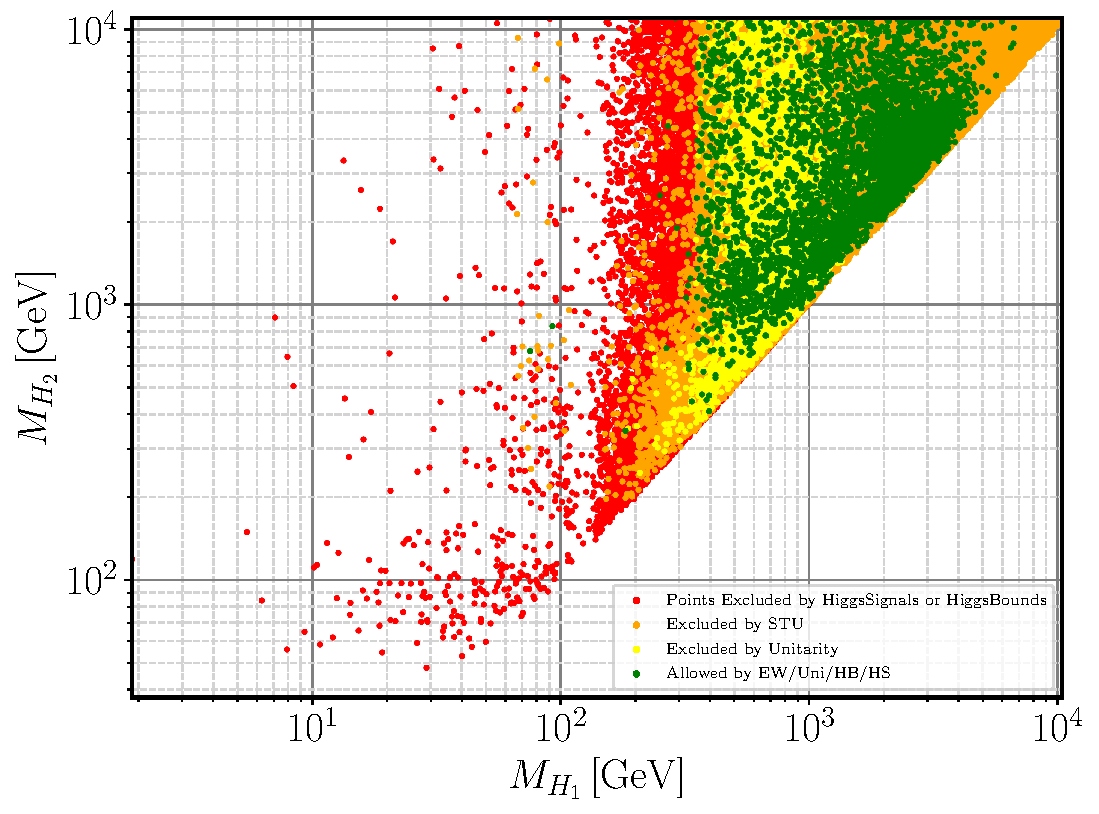
\includegraphics[width=.49\textwidth]{/3HDM/H1_H2.pdf}
	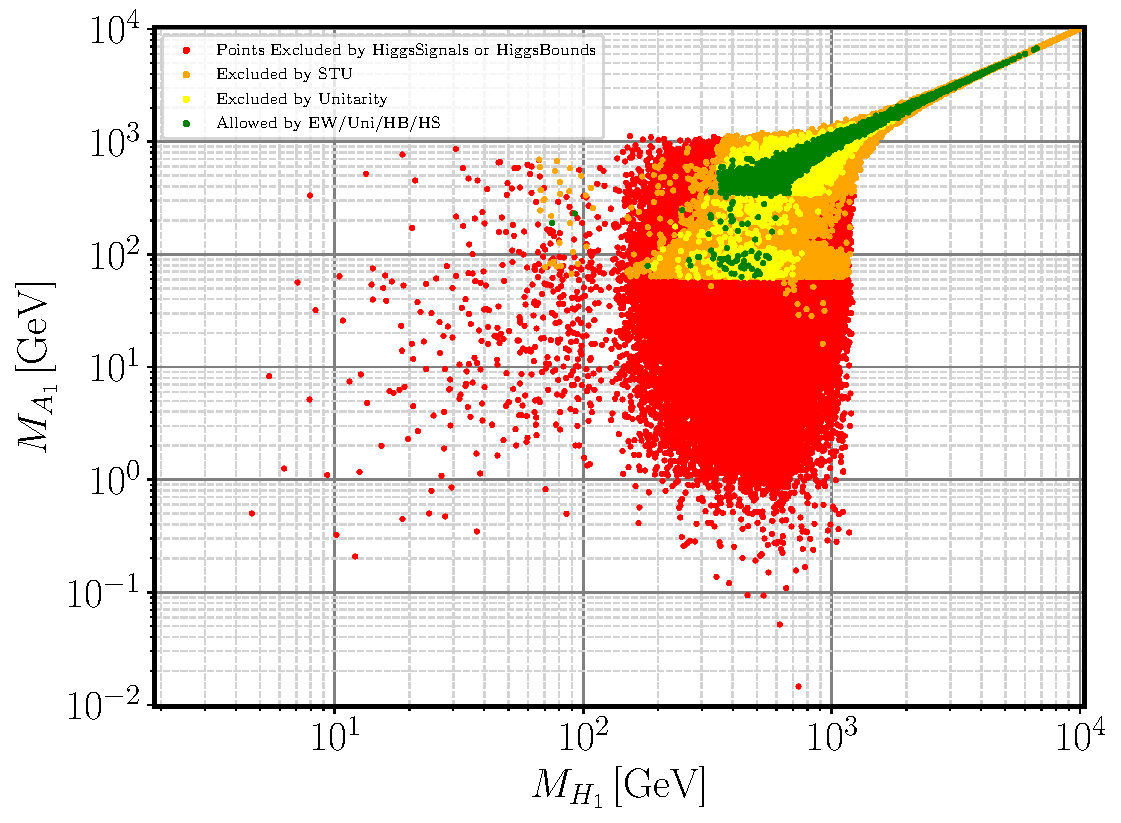
\includegraphics[width=.49\textwidth]{/3HDM/H1_A1.pdf}
	\caption{Scatter plots of parameter space allowed under  several cuts imposed on the BGL-like 3HDM. Right we have the plot showing the masses of the two heavier CP-even scalars $H_2$ and $H_1$ while in the right we show the relation between the lightest
(non-h) of the CP-even and pseudoscalar particles. Red points failed HS and HB tests; yellow points violate unitarity constraints; orange points only fail electroweak precision constraints, and green ones satisfy all restrictions.}
	\label{fig:H1_A1_Plots}
\end{figure}	

\begin{figure}[H]
	\centering
	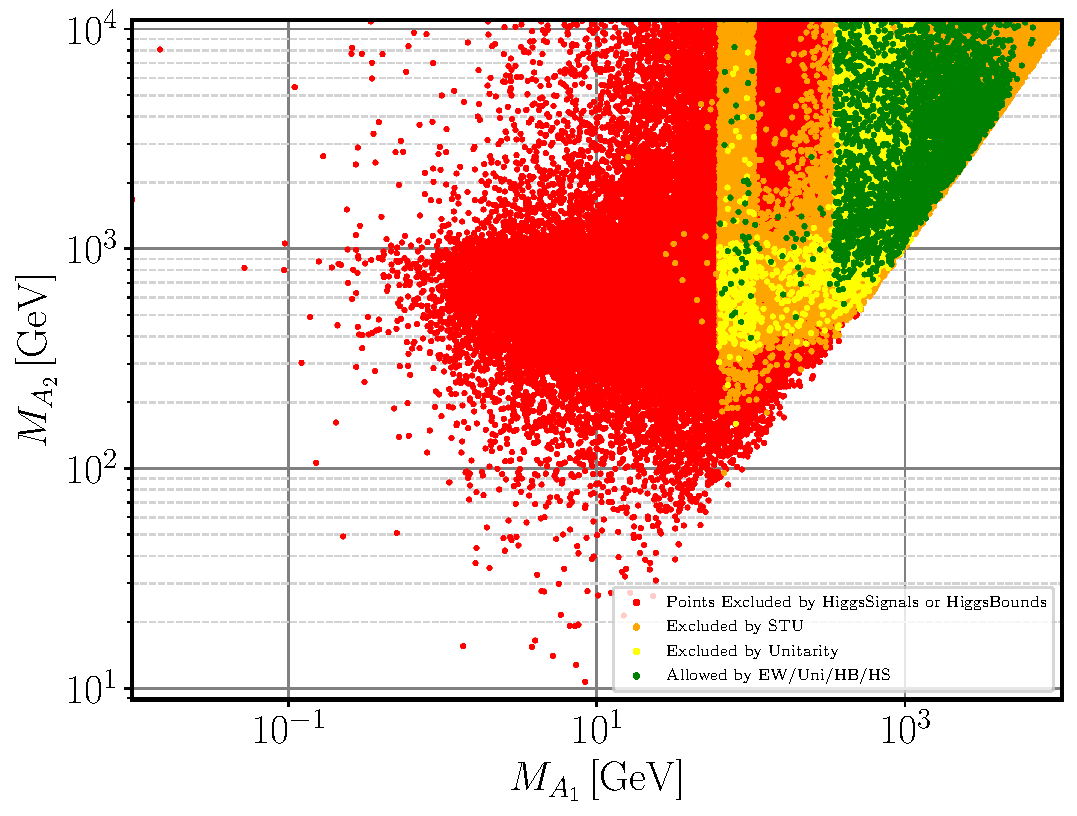
\includegraphics[width=.49\textwidth]{/3HDM/A1_A2.pdf}
	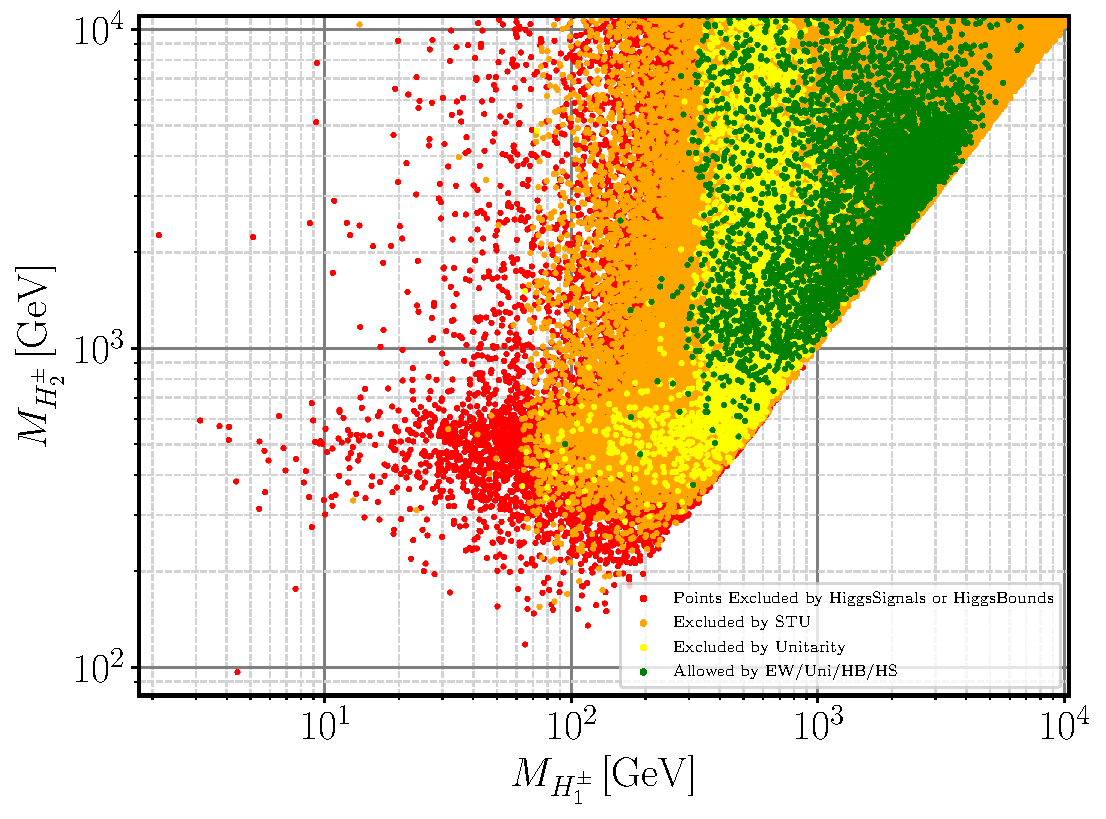
\includegraphics[width=.49\textwidth]{/3HDM/Hc1_Hc2.pdf}
	\caption{}
	\label{fig:Other_H_plots}
\end{figure}	
%
O
%
\subsection{Flavour results}

\begin{figure}[H]
	\centering
	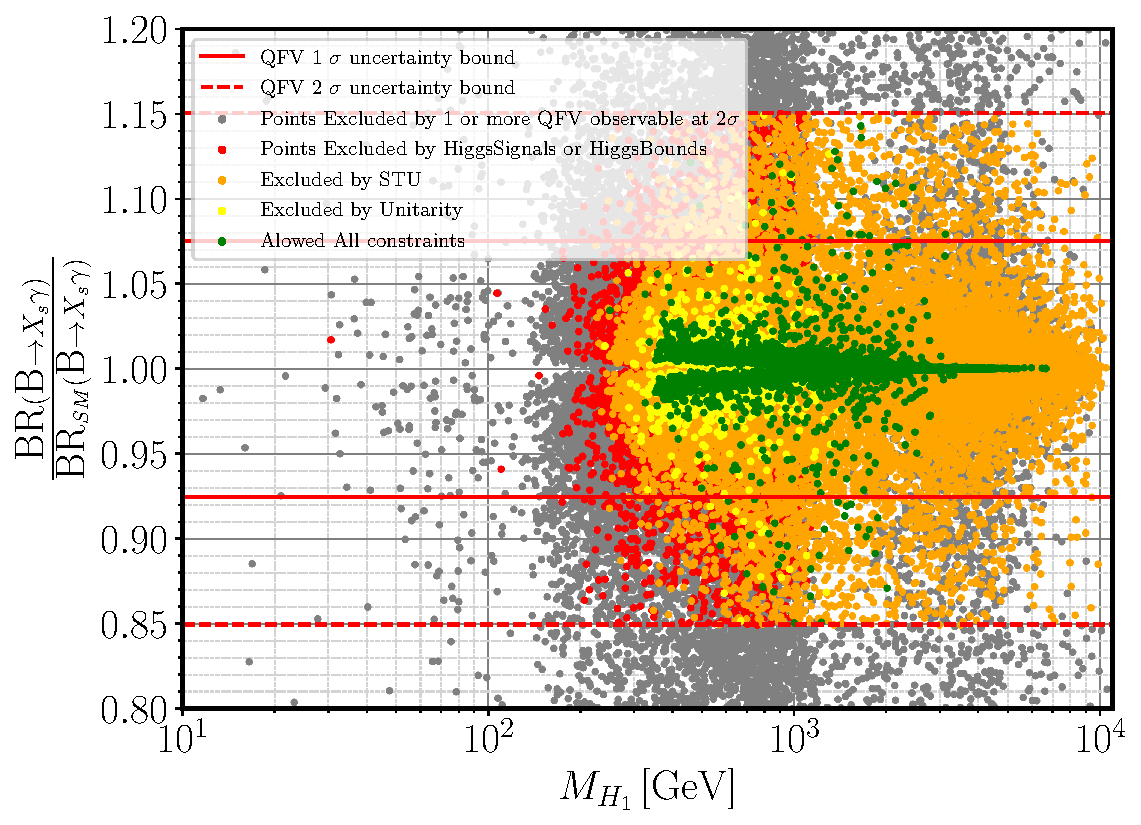
\includegraphics[width=.49\textwidth]{/3HDM/XsGamma_H1.pdf}
	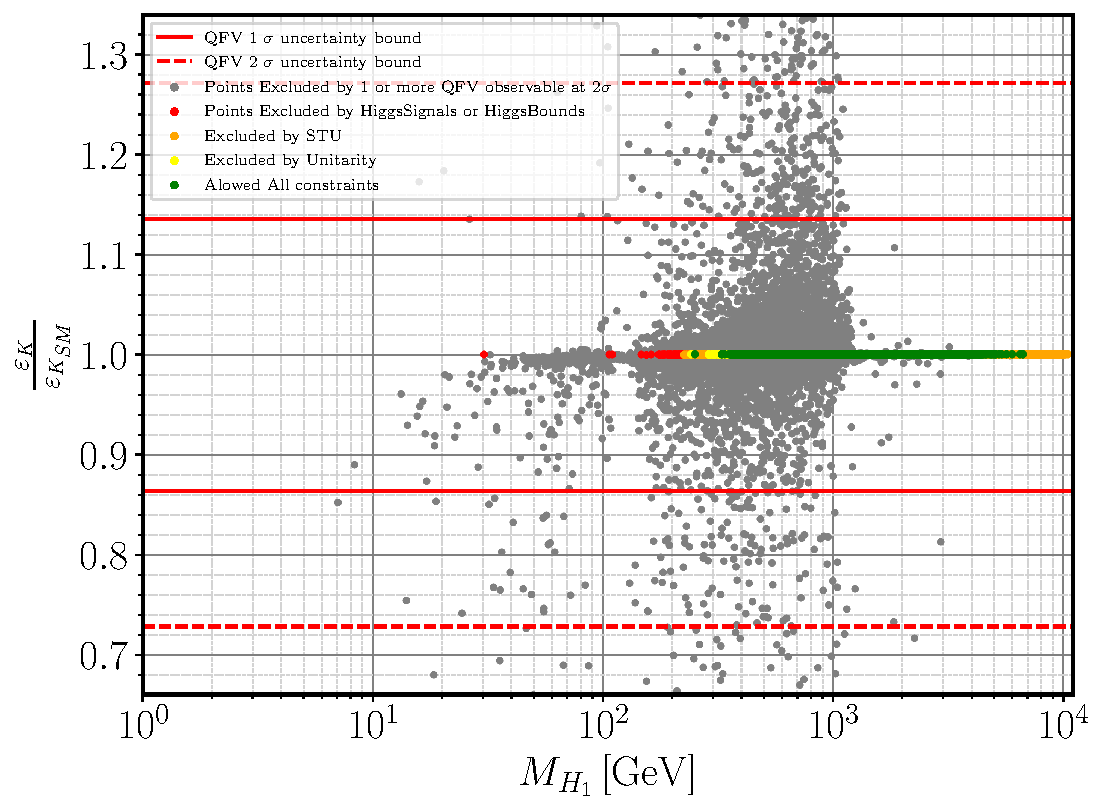
\includegraphics[width=.49\textwidth]{/3HDM/Eps_K_H1.pdf}
	\caption{Scatter plots of parameter space allowed under  several cuts imposed on the BGL-like 3HDM. Right we have the plot showing the masses of the two heavier CP-even scalars $H_2$ and $H_1$ while in the right we show the relation between the lightest
(non-h) of the CP-even and pseudoscalar particles. Red points failed HS and HB tests; yellow points violate unitarity constraints; orange points only fail electroweak precision constraints, and green ones satisfy all restrictions.}
	\label{fig:PT_plots_H1}
\end{figure}	


\begin{figure}[H]
	\centering
	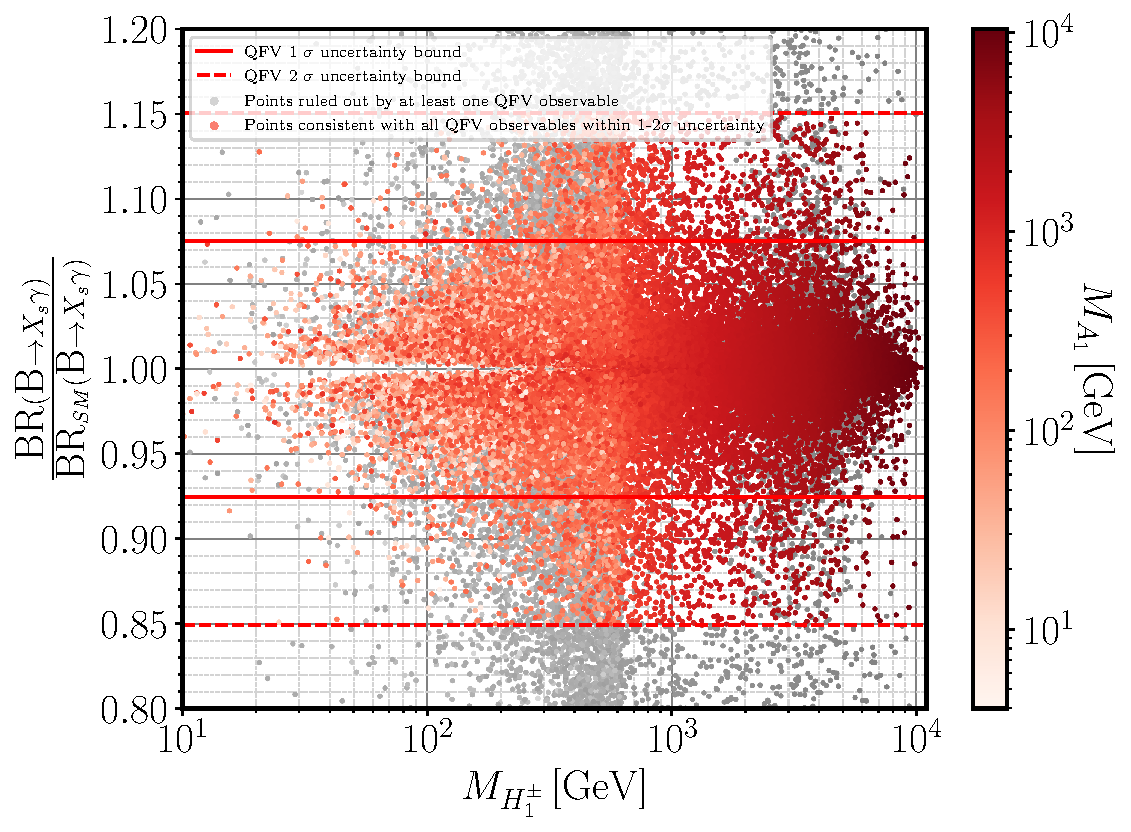
\includegraphics[width=.75\textwidth]{/3HDM/Xsgamma_Hc1_A1.pdf}
	\caption{}
	\label{fig:STU}
\end{figure}	

\begin{figure}[H]
	\centering
	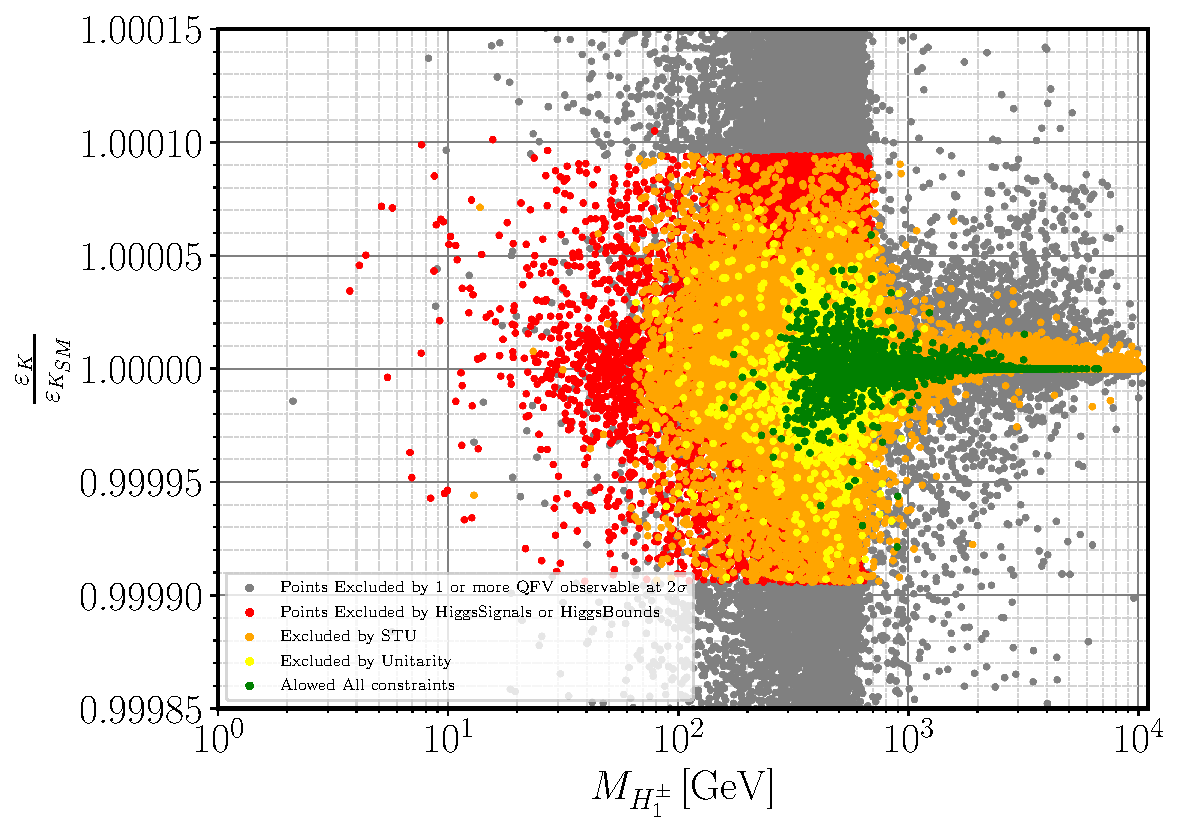
\includegraphics[width=.75\textwidth]{/3HDM/Eps_K_Hc1_Thighter_Centered.pdf}
	\caption{}
	\label{fig:STU}
\end{figure}	

\subsubsection{Fine-Tuning}


\subsection{Conclusions}
 
New scalars with masses below
the TeV scale can still successfully negotiate the constraints arising from flavour data.

\section{Old}

We have studied the main features and the phenomenological  consistency of a family non-universal Three Higgs Doublet Model or 3HDM with a softly broken $\mathrm{U(1)\times Z_2} $ symmetry group. This broken symmetry will justify the flavour hierarchies in the SM and trough a Branco-Grimus-Lavoura mechanism supress the otherwise expected Flavour Changing Neutral Currents. 

Let us now consider an extended version of the SM, with an enlarged Higgs sector that contains three generations of scalar-doublets. These Higgs will be named $\phi^i$ with $i={1,2,3}$.  In this sector we must enforce the alignment limit to the scalar sector ensuring the physical scalar spectrum accommodates a SM-like Higgs boson with mass of $125.09$ GeV.